\chapter{MPI и потоки}
	
	% http://www.mcs.anl.gov/research/projects/mpi/mpi-standard/mpi-report-2.0/node163.htm#Node163
	Процесс в MPI может быть многопоточным. 
	Каждый поток может делать MPI-вызовы, однако потоки не адресуются отдельно: ранг при отправке или получении сообщения идентифицирует процесс, а не поток. 
	Сообщение, отправленное процессу, может быть получено любым потоком в этом процессе.
	 
	 %TODO Возможно, стоит убрать следующий абзац
	Пользователь несет ответственность за предотвращение гонок, когда потоки внутри одного и того же приложения вызывают конфликтующие вызовы связи. 
	Пользователь может убедиться, что два потока в одном и том же процессе не будут вызывать конфликтующие вызовы связи, используя различные коммуникаторы в каждом потоке.
	
	Ниже перечислены два основных требования к реализации, совместимой с потоком. 
	\begin{enumerate}
		\item \textit{Все вызовы MPI являются потокобезопасными.} 
		Например, два одновременно работающих потока могут вызывать вызовы MPI, и результат будет таким, как если бы вызовы выполнялись в некотором порядке, даже если их выполнение чередуется.
		\item \textit{Блокирование вызовов MPI блокирует только вызывающий поток, позволяя выполнять другой поток, если он доступен.} 
		Вызывающий поток будет заблокирован до тех пор, пока не произойдет событие, появления которого он вызывает. 
		Как только событие получено, вызов завершится, и поток будет отмечен как runnable, в течение конечного времени. Заблокированный поток не будет блокировать другие запущенные потоки в одном и том же процессе и не будет препятствовать выполнению MPI выховов.
	\end{enumerate}

	Вызов \textit{MPI\_FINALIZE} должен происходить в том же потоке, который инициализировал MPI. 
	Этот поток называется основным. 
	Вызов метода \textit{MPI\_FINALIZE} должен происходить только после того, как все потоки процессов завершили свои вызовы MPI и не имеют ожидающих сообщений или операций ввода-вывода. 
	Это ограничение упрощает реализацию.
	
	Программа, в которой два потока блокируются, ожидая одного запроса, ошибочна. 
	Аналогично, один и тот же запрос не может появляться в массиве запросов двух одновременных вызовов \textit{MPI\_WAIT\{ANY | SOME | ALL\}}. 
	В MPI запрос может быть выполнен только один раз. 
	Любая комбинация ожидания или теста, которая нарушает это правило, является ошибочной.
	
	\section{Инициализация}
	Следующая функция может использоваться для инициализации MPI и инициализации среды потока MPI вместо \textit{MPI\_INIT}.
	
	\textit{MPI\_INIT\_THREAD(required, provided)}
	
	\textit{IN} required - желаемый уровень поддержки многопоточности (integer)
	
	\textit{OUT} provided - полученный уровень поддержки многопоточности (integer)
	
	Этот вызов инициализирует MPI таким же образом, что и вызов \textit{MPI\_INIT}. Кроме того, он инициализирует среду потока. Аргумент \textit{required} используется для указания желаемого уровня поддержки потоков. Возможные значения перечислены в порядке возрастания поддержки потоков.
	
	\begin{enumerate}
		\item \textit{MPI\_THREAD\_SINGLE} - для однопоточного приложения.
		\item \textit{MPI\_THREAD\_FUNNELED} - Процесс может быть многопоточным, но только один поток может делать MPI-вызовы. Все MPI-вызовы перенаправляются в основной поток.
		\item \textit{MPI\_THREAD\_SERIALIZED} - Процесс может быть многопоточным и многие потоки могут делать MPI-вызовы, но только по одному.
		MPI -вызовы не производятся одновременно из двух отдельных потоков.
		\item \textit{MPI\_THREAD\_MULTIPLE} - Многие потоки могут делать MPI-вызовы без ограничений.
	\end{enumerate}

	Эти значения монотонно возрастают:
	
	$ MPI\_THREAD\_SINGLE < MPI\_THREAD\_FUNNELED < MPI\_THREAD\_SERIALIZED < MPI\_THREAD\_MULTIPLE $.
	 
	Для разных процессов могут потребоваться различные уровни поддержки потоков.
	
	Вызов \textit{MPI\_INIT\_THREAD} возвращает предоставленную информацию о фактическом уровне поддержки потоков, который будет предоставляться MPI. 
	Это может быть одно из четырех значений, перечисленных выше.
	
	Уровень(и) поддержки потоков, который может быть предоставлен MPI\_INIT\_THREAD, будет зависеть от реализации MPI и может зависеть от информации, предоставленной пользователем до начала запуска программы (например, с аргументами mpiexec). 
	Если возможно, вызов будет успешно возвращен при \textit{provided} = \textit{required}. 
	В противном случае вызов вернет максимальный поддерживаемый уровень \textit{provided} > \textit{required} (таким образом, обеспечивающий более высокий уровень поддержки, чем требуется пользователю).
	Наконец, если требование пользователя не может быть удовлетворено, тогда вызов вернёт максимально поддерживаемый уровень.
	
\chapter{Реализация ЯГСПП}
	Ограничение реализации заключается в отсутствии рекурсии. При этом возможны циклы.

	\section{Особенности реализации}
	\begin{itemize}
		\item Модули распределяются между узлами вычислительной сети до начала вычислений. Каждый модуль исполняется только на закреплённом за ним узле сети. Принцип распределения не уточняется. В простейшем случае случайно и равномерно.
		\item На каждом узле существует единственный поток, осуществляющий сообщение по MPI с вычислительной сетью.
		\item Принимаемые сообщения после обработки отправляются в буфер.
		\item Поток-планировщик ГСПП сканирует буфер и определяет модули, готовые к срабатыванию. Для каждого завершённого набора данных запускается нить. 
		\item После выполнения вычислений модуль определяет значения, которые будут переданы другим модулям. Значения отправляются в буфер. С помощью реестра модулей формируются сообщения и, если необходимо, передаются на другие узлы сети через нить MPI.
	\end{itemize}
	
	Важной особенностью такой архитектуры является обособленность управляющей части программы от исполняющей, что позволяет представить общую архитектуру вычислительных узлов подобной вычислительной сети. На рисунке \ref{fig:architecture} изображены основные компоненты. Стрелками показаны направления обмена данными.
	
			\begin{figure*}[h]
				\centering
				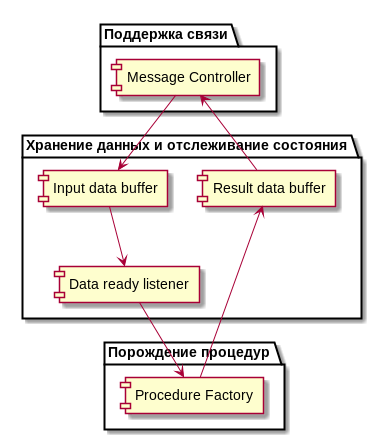
\includegraphics[width=0.5\linewidth]{graph-scheme-cpp-architecture}
				\caption{Общая архитектура вычислительных узлов ЯГСПП}
				\label{fig:architecture}
			\end{figure*}
			
	\FloatBarrier
	
	Легко заметить, что заданные ограничения наложены лишь на компоненты поддержки связи (использование MPI) и на модуль порождения процедур (использование нитей для запуска процедур модулей). Таким образом можно выделить общую часть - компоненту хранения данных и отслеживания состояния, которая может послужить каркассом для построения аналогичных систем. Например, как фреймворк для поддержки связи и порождения процедур можно использовать PVM или микросервисную архитектуру с поддержкой многопоточности.
	
\chapter{Результат реализации}
 Для использования полученной библиотеки необходимо создать наследников класса \textit{\textbf{Procedure}} для каждого модуля, участвующего во взаимодействии.  В листинге ниже приведён пример процедуры, осуществляющей вывод в стандартный поток вывода данных и последующая отправка сообщения модулю 3 на вход 0.
 
 \lstinputlisting[caption={Пример реализации процедуры}]{listings/example-procedure.cpp}
 
 Далее необходимо в функции main проинициализировать модули, указав начальный и конечный модуль

 \lstinputlisting[caption={Пример функции \textbf{main}}]{listings/example-main.cpp}
 
 Модуль может быть одновременно начальным и конечным. Для спецификации такого модуля нужно использовать слияние флагов: $ \text{INITIAL | FINAL} $.
 
 Процедура финального модуля должна сообщать о том, что обработка данных с указанным тегом завершена. Это необходимо для остановки исполняющей программы.
 
 \lstinputlisting[caption={Пример функции \textbf{main}}]{listings/example-final-procedure.cpp}
  
Исходный код проекта доступен на GitHub \href{https://github.com/goto1134/graph-scheme-cpp-mpi}{https://github.com/goto1134/graph-scheme-cpp-mpi}.

\chapter{Пример программы}



	